 \documentclass[a4paper,twoside]{article}

%% Language and font encodings
\usepackage[spanish]{babel}
\usepackage[utf8]{inputenc}
\usepackage[T1]{fontenc}


%% Sets page size and margins
\usepackage[a4paper,top=3cm,bottom=2cm,left=2.5cm,right=2.5cm,marginparwidth=0.5cm]{geometry}

\usepackage{amsmath}			%Paquete matemático
\usepackage{graphicx}
\usepackage[colorinlistoftodos]{todonotes}

\usepackage{hyperref}		%Paquete empleado para colocar hipervinculos
\hypersetup{
	colorlinks = true,
	linkcolor = black,
}

\usepackage{eurosym}
\usepackage{pdfpages}			%Sirve para incluir PDF en el documento
\usepackage{anysize}			%Podremos colocar imagenes de cualquier tamaño
\usepackage{subfig}				%Nos permitira colocar varias imagenes en una figura
\usepackage{float}				%Podremos crear y colocar boxes donee queramos
\usepackage[export]{adjustbox}

%Colocamos cabeceras y pies de pagina
%(CONSULTA: http://edicionesoniricas.com/maquetar-latex-encabezados-pies-pagina/)
%(CONSULTA2: https://es.sharelatex.com/learn/Headers_and_footers)
%\bfseries es análogo a \textbf{}
% \leftmark-> Adds name and number of the current top-level structure (section for article) in uppercase letters.
%\rightmark-> Adds name and number of the current next to top-level structure (subsection for article) in uppercase letters.
\usepackage{fancyhdr}		%Paquetes necesarios
\pagestyle{fancy}			%Borra los parametros por defecto
\fancyhf{}
\fancyhead[RO,LE]{\bfseries\thepage}
\fancyhead[LO,RE]{\bfseries\rightmark}
%Nos aseguramos de que en las paginas plain, no haya ni cabeceras ni lineas
\fancypagestyle{plain}
{
	\fancyhead{} % elimina cabeceras en paginas "plain"
	\renewcommand{\headrulewidth}{0pt} % así como la raya
}

%Definimos las lineas divisoras de las cabeceras y pie de pagina
\renewcommand{\headrulewidth}{1pt}	%Define el grosor de la línea de head
\renewcommand{\footrulewidth}{0pt}		%Define el grosor de la linea foot (Si no queremos linea, 0pt)
\addtolength{\headheight}{0.5pt} % espacio para la raya

%Librerias para introducir código de Matlab
%\usepackage{bigfoot} % to allow verbatim in footnote
\usepackage[numbered,framed]{matlab-prettifier}

\lstset{
	style              = Matlab-editor,
	basicstyle         = \mlttfamily,
	escapechar         = ",
	mlshowsectionrules = true
}

% %%%%%%%%% INTRODUCIR CODIGO DE C %%%%%%%%%%%%%%%%%%%%%%
\usepackage{listings}
\usepackage{xcolor} % for setting colors

% set the default code style
%:Paquete para modificar los colores de diferentes elementos del codigo

\definecolor{mGreen}{rgb}{0,0.6,0}
\definecolor{mGray}{rgb}{0.5,0.5,0.5}
\definecolor{mPurple}{rgb}{0.58,0,0.82}
\definecolor{backgroundColour}{rgb}{0.95,0.95,0.92}

%Definimos el estilo del codigo de C
\lstdefinestyle{CStyle}{
	backgroundcolor=\color{backgroundColour},
	commentstyle=\color{mGreen},
	keywordstyle=\color{magenta},
	numberstyle=\tiny\color{mGray},
	stringstyle=\color{mPurple},
	basicstyle=\footnotesize,
	breakatwhitespace=false,
	breaklines=true,
	captionpos=b,
	keepspaces=true,
	numbers=left,
	numbersep=5pt,
	showspaces=false,
	showstringspaces=false,
	showtabs=false,
	tabsize=2,
	language=C,
}
% %%%%%%%%%%%%%%%%%%%%%%%%%%%%%%%%%%%%%%%%%%%%%%%%%%

% Pie de pagina
%\fancyfoot{} % limpia el pie
\fancyfoot[C]{- \thepage -} % número de página centrado

%Nos generará texto para pruebas de maquetado
\usepackage{lipsum}

% To include code
\usepackage{minted}
%\usemintedstyle{borland}
% To can use multirow
\usepackage{multirow}

% Se varia el limite de colimnas de latex
\setcounter{MaxMatrixCols}{11}
\usepackage{lscape}
%----------------------------------------------------------------------------------------------------------------------------------
\begin{document}
\begin{titlepage}
 \centering
 \Huge{\textbf{SISTEMAS ELECTRÓNICOS PARA LA AUTOMATIZACIÓN}} \\
 \Huge{\textit{Proyecto de microcontroladores}}\\

 \vspace{1cm}
 \LARGE{Grado en Ingeniería Electrónica, Mecatrónica y Robótica}\\
 \rule{\textwidth}{0.1mm}
 % \begin{figure}[h!]
 %	\centering
 %	\includegraphics[width=.5\textwidth]{fpga}
 %	% \caption{Placa de desarrollo}
 % \end{figure}

 \vspace{2cm}
 \rule{\textwidth}{0.1mm}
 \Large{\textbf{Autores:} Haes-Ellis, Richard Mark\\
 Montes Grova, Marco Antonio}
\end{titlepage}
\tableofcontents
\newpage

% %%%%%%%%%%%   INTRODUCCION %%%%%%%%%%%%%%%%%%
\section{Introducción al proyecto}
En este proyecto, se desarrollara un HID(\textit{Human Interface Device}) el control del puntero de un host, en este caso un ordenador, haciendo  uso del Boosterpack \textit{BOOSTXL-SENSORS} y el microcontrolador \textit{Tiva TM4C1294}, ambos del fabricante \textit{Texas Instruments}.\\
En primer lugar, se realizará una introducción al hardware empleado en el mismo para, posteriormente, abordar el software. Tras ello, en los siguientes puntos del proyecto, se trataran aspectos como el funcionamiento a alto nivel del proyecto como los códigos implementados en propio microcontrolador.\\
En un ultimo apartado se trataran futuras o posibles mejoras y sus posibles aplicaciones a la automatizacion industrial.
\subsection{Descripcion del hardware empleado}
Se ha empleado como placa de desarrollo del proyecto el modelo TM9C1294 de la serie Tiva C de Texas Instrument. Este microntrolador es el que se muestra a continuación: \\
 \begin{figure}[h!]
	\centering
	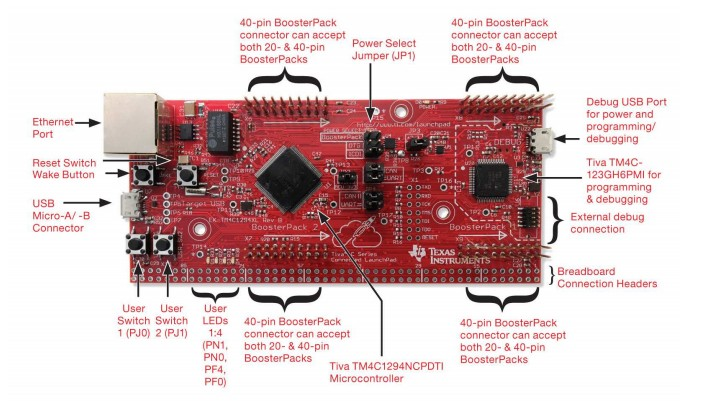
\includegraphics[width=.7\textwidth]{../images/tiva_tm4c1294}
  \caption{Microcontrolador empleado en el proyecto}
\end{figure}

Como se puede observar, ademas de poseer una conexion Ethernet, USB y una serie de leds, tendra un microcontrolador integrado, el Tiva TM123GH, conectado a un puerto USB cuya funcionalidad sera programar el microcontrolador principal. \\
Ademas de ello, dispone de dos pares de ristras de pines destinadas al conexionado de dos Boosterpacks distintos, de tal modo que se puedan ampliar las funcionalidades como pueden ser una pantalla o el boosterpack empleado en este proyecto, BOOSTXL-SENSORS. \\

Para conocer informacion adiccional sobre el microcontrolador implementado en la placa puede la guia propocionada por el fabricante: \url{http://www.ti.com/lit/ug/spmu365c/spmu365c.pdf}. \\

Se ha optado por el uso de este microcontrolador para este proyecto por su capacidad de .......... lo de poder controladr el raton........
\newpage

En cuanto al Boosterpack empleado, BOOSTXL-SENSORS, es el mostrado a continuacion: \\
\begin{figure}[h!]
 \centering
 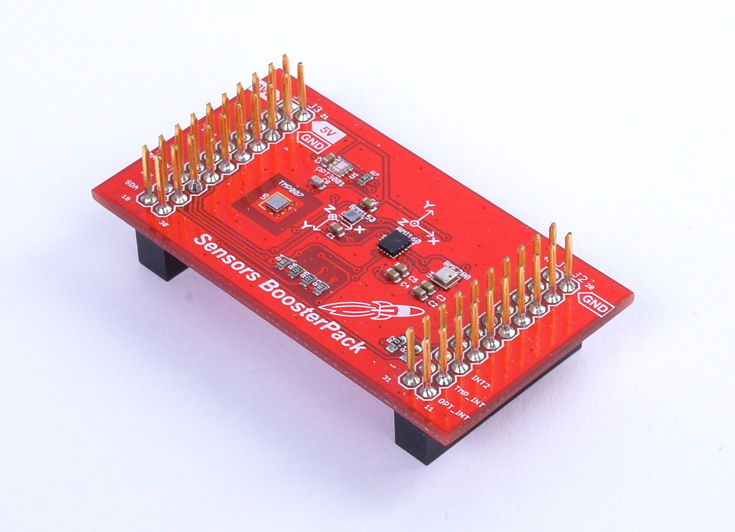
\includegraphics[width=.3\textwidth]{../images/sensors_bp}
 \caption{Boosterpack empleado en el proyecto}
\end{figure}

contiene una gran cantidad de sensores como son una IMU, un magnetometro, sensores ambiente y de luminosidad y sensor de temperatura. En lo que a este proyecto respecta, el principal sensor que se empleara sera la IMU integrada, la \textit{BMI160} de 6 ejes, es decir, se encuentra formada por un acelerometro de 3 ejes y un giroscopio de 3 ejes. \\

La medida del acelerometro sera dada en \textit{g}, la cual puede ser estimulada modificando la orientacion respecto a la gravedad de la tierra, o cambiando la velocidad a lo largo de un eje. En cuanto a la medida del giroscopio sera dada en grados por segundo, la cual se estimulara girando la placa respecto sus ejes absolutos. \\
En este proyecto, se emplearan las medidas asociadas a las velocidades angulares en torno a los ejes X y Z, ya que son las unicas empleadas para posicionarse en el plano 2D que forma la pantalla del computador. Se mostrara a continuacion una imagen en la cual se mostrara el movimento en torno al eje X que generara una variacion de la velocidad angular medida por el giroscpio:\\
\begin{figure}[h!]
 \centering
 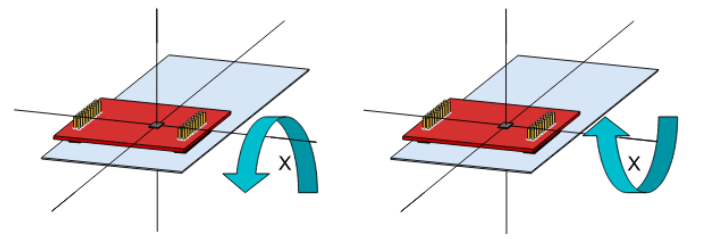
\includegraphics[width=.6\textwidth]{../images/mov_axisX_bmi}
 \caption{Movimento en torno al eje X que genera una variacion de velocidad angular}
\end{figure}

La variación del angulo en torno al eje Z se medira del mismo modo, como se muestra a continuación: \\
\begin{figure}[h!]
 \centering
 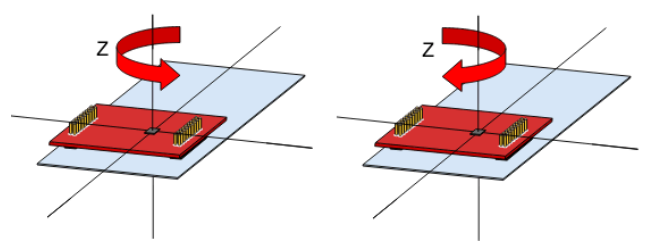
\includegraphics[width=.6\textwidth]{../images/mov_axisZ_bmi}
 \caption{Movimento en torno al eje Z que genera una variacion de velocidad angular}
\end{figure}

\newpage
La comunicación del sensor con otros sensores del boosterpack y con la placa sera por medio de $I^2C$, el cual es el principal bus serie de datos, empleado para la comunicación entre elementos de un circuito. \\

Al igual que antes, se puede consultar datos concretos de cada sensor en la guia proporcionada por el fabricante:
\url{http://www.ti.com/lit/ug/slau666b/slau666b.pdf}

\subsection{Descripcion del software empleado}
En cuanto al software empleado se basara en la API proporcionada por el fabricante, \textit{TivaWare} para la familia de microcontoladores TIVA. Esta API contiene los elementos que se muestran en la siguiente imagen:\\
\begin{figure}[h!]
 \centering
 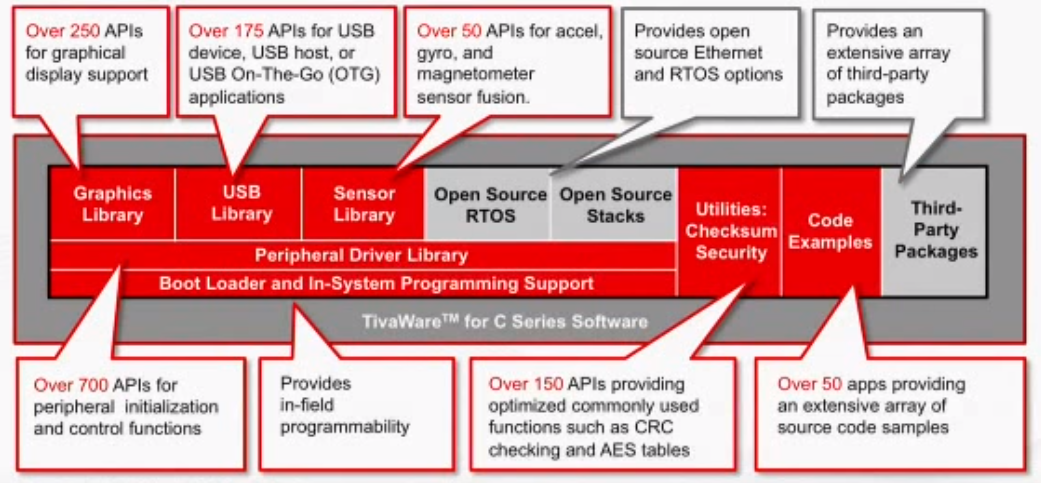
\includegraphics[width=.8\textwidth]{../images/tivaware_struct}
 \caption{Estructura de la API Tivaware}
\end{figure}

Principalmente, se emplearan las liberias asociadas al manejo de los perifericos, \textit{Peripheral Driver Library}, al manejo del puerto USB,\textit{USB Library} y al manejo de sensores,\textit{Sensor Library}. \\
Ademas de la gran ayuda brinda la API, se proporcionan una serie de ejemplos de uso que ayudaran al desarrollo del software propio. \\

Ademas de ello, ha sido necesario el uso de librerias para el manejo de los GPio de la placa y la comunicacion por el puerto serie de la UART. \\
Ademas de ello, se han empleado una serie de declaraciones proporciondadas por el profesor para solventar el desajuste de la actualizacion de las librerías, \textit{driverlib2.h} y \textit{sensorlib2.h}.

\newpage
\section{Funcionamiento del proyecto}
En este apartado, se desarrollarán las principales funcionalidades implementadas en el proyecto. Las principales funciones son:
\begin{itemize}
\item Desarrollo de un HID con el microcontrolador.
\item Empleo del Boosterpack para tomar la definir la posicion del puntero en la pantalla.
\item Filtrado de las medidas tomadas a nivel de software.
\end{itemize}

Un HID(\textit{Human Interface Device}) es una arquitectura de comunicacion empleada para comunicar los perifericos de interaccion humana como pueden ser ratones o teclados.\\
La comunicación entre el dispositivo HID y el host se realiza a través de un conjunto de estructuras de "informes" definidas por el dispositivo que el host puede consultar. Los informes se definen tanto para la comunicación de la entrada del dispositivo con el host y para la selección de salidas y funciones del host. \\

Además de la flexibilidad que ofrece la arquitectura básica, los dispositivos HID también se benefician de una gran universalidad entre sistemas operativos, lo que significa que no es necesario desarrollar un driver, sobre todo en el caso de dispositivos estándar como teclados y joysticks.\\
A pesar de estas ventajas, el uso de HID tiene un inconveniente. La tasa de datos que pueden transferirse esta limitada a un máximo de 64 KB/s.\\

Se empleara comunicacion mediante USB. El puerto USB de la familia Tiva TM4C de microcontroladores soporta 3 modos de funcionamiento:
\begin{itemize}
	\item \textbf{Host mode}: Permite conectar un teclado o un raton al microcontrolador.
	\item \textbf{Device mode}:Establece una comunicacion con el PC a traves del USB.
	\item \textbf{On-The-Go mode}: Permite multiplexar el USB entre hosts y dispositivos.
\end{itemize}
En este proyecto se empleara el USB en modo \textit{Device} o dispositivo, ya que se busca controlar el puntero del ordenador con el microcontrolador.\\
Durante el desarrollo del codigo de programacion se detallara el modo en el que se establece esta comunicacion entre el ordenador y el microcontrolador por medio del USB para crear el HID buscado. \\

Por otro lado, para controlar la posicion del puntero en la pantalla, se hara uso del giroscopio que, empleando la velocidad angular obtenida por el mismo, se podra estimar la posicion del puntero en el plano de la pantalla a partir de la definicion de un sistema inicial. \\
Como se mostro cuando se explico el boosterpack empleado que contiene el sensor, se tomaran las medidas de la velocidad angular en torno a los ejes X y Z. \\

\section{Código de programación desarrollado}
En primer lugar, es conveniente mostrar un esquema de las librerias y funciones empleadas en el proyecto. Ese esquema se muestra a continuacion:


\newpage
En el codigo principal, es decir, en \textit{usb\_dev\_mouse.c}, en primer lugar se hara la declaracion de librerias. Las primeras librerias que se declararan son las asociadas a las funciones logicas del microntrolador.

\begin{listing}[h!]
\inputminted[linenos,breaklines,frame=lines,framesep=2mm]{c}{codes/variables.c}
\caption{Variables y defines del codigo}
\end{listing}

\begin{listing}[h!]
\inputminted[linenos,breaklines,frame=lines,framesep=2mm]{c}{codes/librerias.c}
\caption{Declaración de librerías}
\end{listing}

\begin{listing}[h!]
\inputminted[linenos,breaklines,frame=lines,framesep=2mm]{c}{codes/funciones.c}
\caption{Funciones empleadas}
\end{listing}

\begin{listing}[h!]
\inputminted[linenos,breaklines,bgcolor=lightgray,frame=lines,framesep=2mm]{c}{codes/main.c}
\caption{Programa principal}
\end{listing}


\newpage
\section{Posibles mejoras del proyecto}
En cuando a la principal mejora del proyecto, se basara en la implementación de una comunicación inalambrica en el mismo. Durante el desarrollo del proyecto se plantearon diversas vias posibles de implementacion:
\begin{itemize}
\item Implementación de una comunicación basada en radio-frecuencia. Esta via se planteo empleando el boosterpack del fabricante \textit{Texas Instrument}, CC110L, el cual emplea el protocolo de comunicacion SimpliciTI. Sin embargo, este modulo de radio frecuencia, ha sido disenado para su utilizacion con el microcontrolador MSP430, y es poco compatible con otros microcontroladores, aunque sea del mismo fabricante. \\
\begin{figure}[h!]
 \centering
 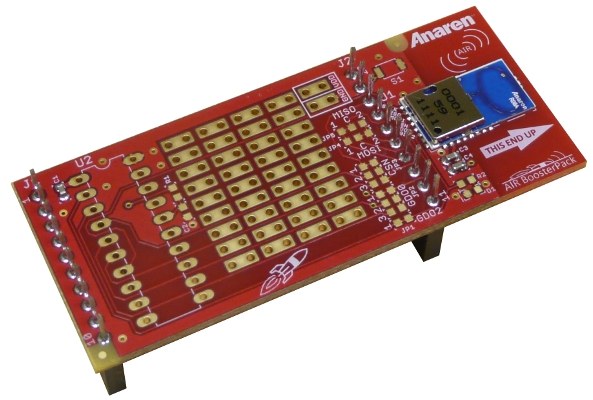
\includegraphics[width=.3\textwidth]{../images/rf_bp}
 \caption{430BOOST-CC110L Boosterpack}
\end{figure}

\item Implementacion de una comunicacion Wi-Fi. Para la implementacion de este modo de comunicacion, se haria uso del modulo ESP01, el cual es un modulo Wi-Fi de bajo coste, que puede ser configurado como punto de acceso o como cliente y enviar mensajes TCP entre varios para comunicarse entre ellos. \\
\begin{figure}[h!]
 \centering
 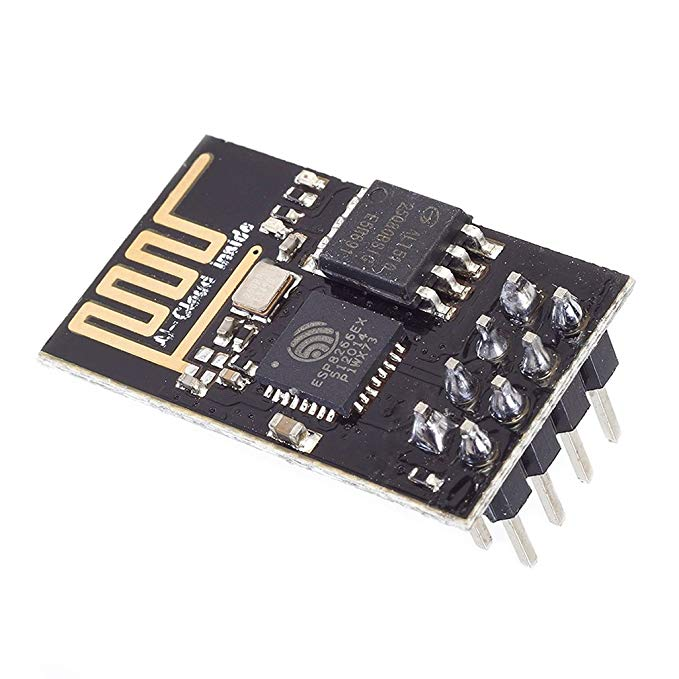
\includegraphics[width=.2\textwidth]{../images/esp8266}
 \caption{Modulo WiFi ESP01}
\end{figure}
\end{itemize}

Esta ultima via de comunicacion, es la que se ha considerado mas factible ya que los modulos ESP01 emplean comandos AT, es decir, el conjunto de comandos Hayes, los cuales son un conjunto de comandos empleados para configurar y parametrizar los modems. \\
La comunicacion del modulo ESP01 es mediante UART(\textit{Universal Asynchronous Receiver-Transmitter}), y debido a que el microntrolador posee 8 puertos UART, es una aplicación bastante factible. Empleando las funciones para enviar datos por la UART en función de la dirección base de la misma, las cuales se encuentran ya diseñadas en el directorio raiz de este proyecto, seria posible establecer una comunicacion serial con el modulo Wi-Fi. Sin embargo, una vez establecida dicha comunicación serial, la cual conlleva consigo una sincronizacion de relojes entre las UART y la comunicación USB para implementar el dispositivo. \\
Una vez establecida esta comunicación, es necesario trazar un entramado de conexiones de red para crear un servidor TCP en el ESP01 a modo de punto de acceso al cual se pueda conectar el otro, el cual se encuentra en el otro microcontrolador, de tal modo que le envíe los datos por tramas TCP asociados a la IMU y la pulsación de los botones.\\

No se ha optado por implementarlo en este proyecto, debido a la necesidad del uso de los objetos inherentes al lenguaje de programacion C++ y sus clases para establecer un buen entramado de conexiones de red. Además de ello presentó una notable carga de tiempo de trabajo la sincronización de los relojes. \\

\newpage

\section{Anexos}

\begin{lstlisting}[language=C,style=CStyle, caption={Declaración e inicialización de variables}]

\end{lstlisting}
\end{document}
